\subsection{Support Vector Machine - SVM \cite{SVm1} }
Support Vector Machine est un classeur discriminant qui est défini par un hyperplan , étant donné un ensemble d'apprentissage l'algorithme de SVM permet de trouver un hyperplan qui va catégoriser les éléments de l'ensemble et d'autres nouveaux éléments en maximisant la marge entre les élements de l'ensemble d'apprentissage  à la manière de la frontière de décision pour la régression logistique. On peut dire que SVN est une amélioration de la régression logistique .
\subsubsection{Données Séparables linéairement }
Si nous considérons le même problème de classification binaire que celui de la régression logistique sauf que les label de nos classe ici sont 1 et -1 au lieu de 0 et 1 donc ici y $\in$ \{-1,1\} , on constate que nous avons un large variétés des choix pour notre frontière de décision  comme on peut le voir à la figure ci dessous :
\begin{figure}[ht]
	\centering
	\subfloat[]{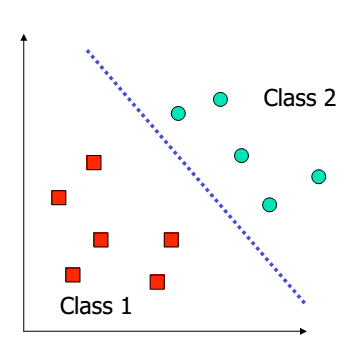
\includegraphics[width=0.3\textwidth]{fig/SVNDecisionBoundary1.png}\label{fig:Image13a}}
	\hfill
	\subfloat[]{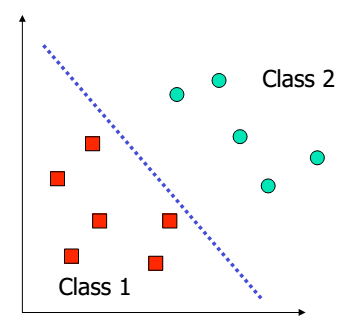
\includegraphics[width=0.3\textwidth]{fig/SVNDecisionBoundary2.png}\label{fig:Image13b}}
	\hfill
	\subfloat[]{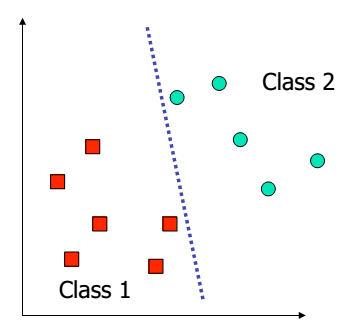
\includegraphics[width=0.3\textwidth]{fig/SVNDecisionBoundary3.png}\label{fig:Image13c}}
	\caption{Différentes frontières de décision possibles }
\end{figure}
Nous remarquons que toutes ces frontières des décisions conviennent pour notre ensemble d'apprentissage.\\ Mais comment alors choisir la bonne?? celle qui est optimale?\\
Remarquons que pour mieux généraliser les données la meilleur  frontière de décision est celle qui doit être le plus éloigné que possible des nos données .  
Le but de SVM revient à trouver cette hyperplan qui constituerai notre frontière de décision.
\paragraph{Représentation de l'hypothèse }
Rappelons que pour la régression logistique notre hypothèse s'écrivait de la manière suivante :
\begin{center}
	${h}_{\theta}\left(x\right)=g({\theta }^{T}{x})$
\end{center} Avec $g(z)$ étant définit comme la fonction sigmoïde.\\
On a aussi fait remarquer qu'on utilise l'équation de la frontière  de décision qui est $({\theta }^{T}{x})$ pour effectuer la classification.
et de la on déduit que les données de la classe positif vérifierons l'équation ${\theta }^{T}{x} > 1$ et les autres ${\theta }^{T}{x} <-1$ .\\
Ainsi la limite de la classe positif est l'hyperplan d'équation  ${\theta }^{T}{x} = 1$  et celle des négatifs est ${\theta }^{T}{x} =-1$ si on tient compte de b comme distance avec l'origine ces droites s'écriront 
${\theta }^{T}{x} + b = 1$  et ${\theta }^{T}{x} + b=- 1$ .
 \begin{figure}[ht]
 	\centering
 	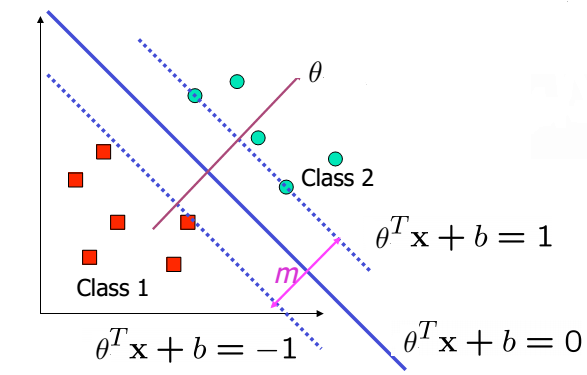
\includegraphics[width=0.5\textwidth]{fig/SVN2D.png}
 	\caption{Problème de SVM en 2 dimesions  }
 	\label{fig:image14}
 \end{figure}\\
Ainsi le but de SVM serait de trouver l'hyperplan qui maximise la marge ou la distance  entre ces 2  hyperplans, et d'après la géométrie analytique cette distance se calcule de la manière suivante $d =\frac{2}{||\theta||}$
Notre problème se formulerait de la manière suivante :
\begin{center}
	$ \left\{\begin{array}{ll}
	max  \frac{2}{||\theta||} ,&  \\
     \mbox{Avec } {\theta }^{T}{x} + b > 1	, & \mbox{si } y\mbox{=1} \\
          \mbox{et  } {\theta }^{T}{x} + b < -1	, & \mbox{si } y\mbox{=-1} 
	\end{array}\right.$
\end{center}
Or maximiser $\frac{2}{||\theta||}$ revient simplement à minimiser $ \frac{1}{2}\theta$
et nos 2 conditions peuvent se combiner en une seule qui est ${y}_{i}({\theta }^{T}{x}_{i} + b )\geq 1 $  $\forall i $ \\
Ainsi le problème à résoudre devient le suivant :
\begin{center}
	$ \left\{\begin{array}{ll}
	min  \frac{1}{2} {||\theta||} ,&  \\
	{y}_{i}({\theta }^{T}{x}_{i} + b )\geq 1, &  \mbox{ $ \forall i$ } \\
	\end{array}\right.$
\end{center}
Ceci n'est rien d'autre qu'un problème d'optimisation sous contrainte, pour le résoudre on utilise la méthode de Lagrange .\\
Elle consiste à cherche le lagrangien de notre problème et égaliser son gradient à zéro.\\
le lagrangien est donné par : 
\begin{center}
 $ {\Large L} = \frac{1}{2} {\theta}^{T} \theta + \sum _{i=1}^{m}{\alpha}_{i}(1-{y}_{i}({\theta }^{T}{x}_{i} + b ))$
 , car  $|| {\theta}||^{2} = {\theta}^{T} \theta $ 
\end{center} 
et ${\nabla }{L}=0$ \\
Ce qui nous donnent : \\
$\frac{\partial L}{\partial {\theta}} =  \theta -  \sum _{i=1}^{m}{\alpha}_{i}{y}_{i}{x}_{i} =0$   ce qui donne  $\theta =  \sum _{i=1}^{m}{\alpha}_{i}{y}_{i}{x}_{i}$\\
$\frac{\partial L}{\partial {b }} =0 $ nous donne $\sum _{i=1}^{m}{\alpha}_{i}{y}_{i}=0 $ \\
En mettant ces 2 expressions des L on obtient : \\
${\Large L} =\frac{-1}{2} \sum _{i=1}^{m} \sum _{i=j}^{m} {\alpha}_{i}{\alpha}_{j}{y}_{i}{y}_{j} {X}_{i}^{T} . {{X}_{j}}+ \sum _{i=1}^{m} {\alpha}{i} $ \\
  ,qui n'est qu'une fonction de ${\alpha}_{i}$ \\
Il est connu sous le nom d'un problème de dualité car si on connait ${\alpha}_{i}$ on connait ${\theta}$  
L doit être maximiser maintenant , ainsi notre problème de dualité s'écrira :\\
\begin{center}
	$ \left\{\begin{array}{ll}
	max \sum _{i=1}^{m} {\alpha}{i} -  \frac{1}{2} \sum _{i=1}^{m} \sum _{i=j}^{m} {\alpha}_{i}{\alpha}_{j}{y}_{i}{y}_{j} {X}_{i}^{T} . {{X}_{j}},&  \\
	\mbox{Avec } \sum _{i=1}^{m}{\alpha}_{i}{y}_{i}=0 , & \\
	\mbox{et }{\alpha}_{i} \ge 0 
	\end{array}\right.$
\end{center}
Avant de s'attaquer à la résolution de ce problème remarquons quelque éléments intéressants qu'il présente :\\
-  la grande partie des valeurs de ${\alpha}_{i}$ sont nulles et  aux    valeurs non nulles correspondent des ${x}_{i}$ qu'on appelle support Vector.\\
-  Pour prédire la classe d'un  nouveaux élément z nous avons qu'a verifer s'il se place au dessus ou en dessous de notre frontière de décision qui est donnée par ${\theta }^{T}{z} + b =  \sum _{i=1}^{m}{\alpha}_{i}{y}_{i}({X}^{T}_{i}.Z) $. \\
- Mais aussi il présente l'avantage que l'algorithme comprend le produit scalaire des tuples d'entrés , cet avantage sera utilisé lorsqu'on va traiter des frontières de  décisions non linéairement séparable.
\subsubsection{Données non Séparables linéairement : Notion de Kernel  \cite{SVm2}}
Dans la plupart des cas surtout dans la pratique les données ne peuvent pas toujours être classer avec une droite ou un hyperplan comme on peut le voir à la \figurename{15} :
 \begin{figure}[ht]
 	\centering
 	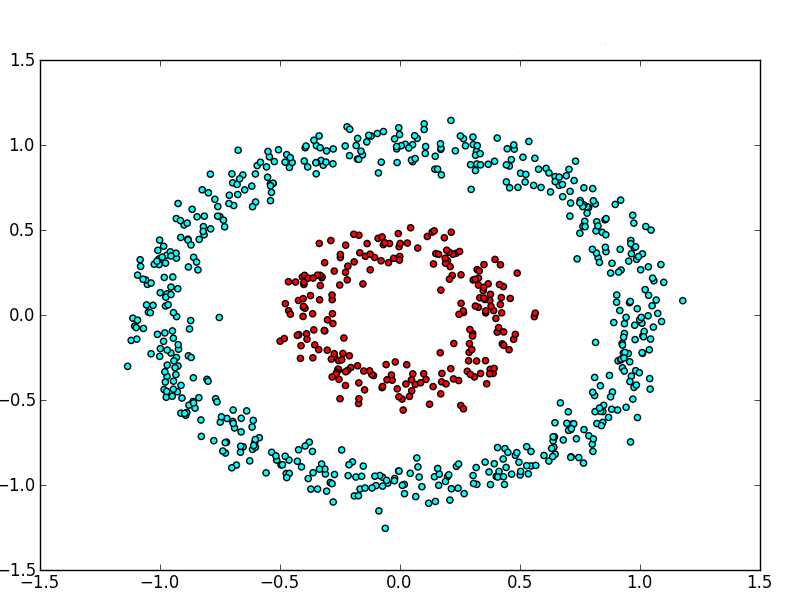
\includegraphics[width=0.5\textwidth]{fig/NonLinearDecisionBoudary.png}
 	\caption{Données non séparable linéairement  }
 	\label{fig:image15}
 \end{figure}\\
 Une propriété stipule que les données qui ne sont pas linéairement séparable dans un espace de dimension n le seront dans un espace de dimension m avec $m \ge n$ \cite{8}. il suffit juste de faire un mapping des tuples ${x}_{i}$  dans ${R}^{n}$ vers ${R}^{m}$ en utilisant une fonction $\phi(x)$. Voyons un exemple à la \figurename{16}\\
  \begin{figure}[ht]
  	\centering
  	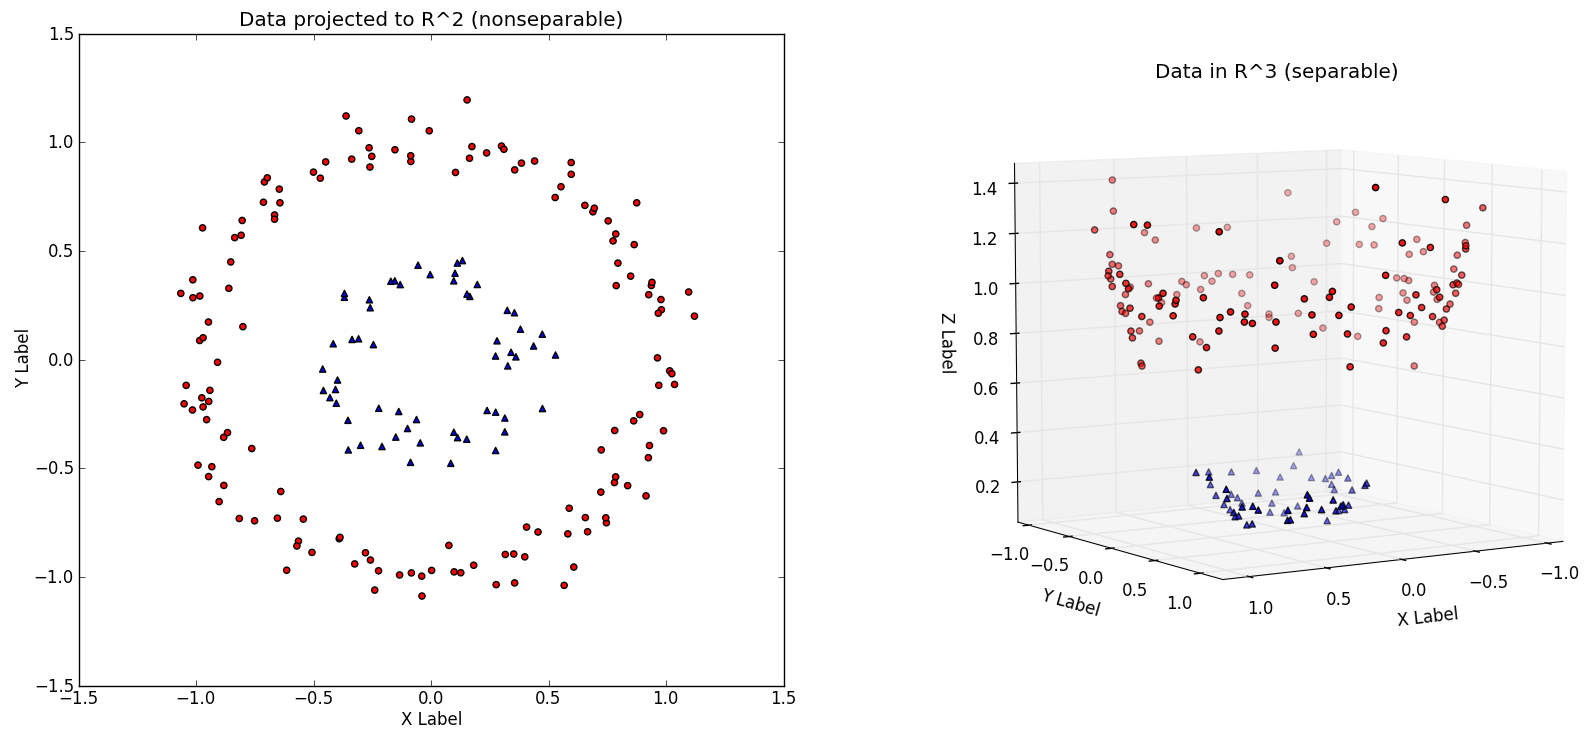
\includegraphics[width=0.5\textwidth]{fig/NonLinearDecisionBoudary2.png}
  	\caption{Données non séparable linéairement dans ${R}^{2}$ mais qui le devient dans ${R}^{3}$ avec $\phi({x}_{1},{x}_{2} ) = ({x}_{1},{x}_{2},{x}^{2}_{1}+{x}^{2}_{2})$ }
  	\label{fig:image16}
  \end{figure}\\
 \emph{\textbf{Définition  : Kernel}}
 Un Kernel est une fonction qui permet de calculer le produit scalaire du mapping d'un tuple dans un espace de dimension supérieur que celui dans lequel il est définie .
 on a : \\
 \begin{center}
 	${\large K }(x,z ) = {\phi}^{T}(x).{\phi}(z)$
 \end{center} 
 Mais on n'est pas obligé de connaitre ${\phi}(x)$ pour calculer ${\large K }(x,z ) $ il existe des Kernel bien définie qui permettent de calculer le produit scalaire sans pour autant connaitre $\phi$ et ainsi faciliter les calcul .\\
 En voici quelque uns les plus utilisé: \\
 - Le Kernel Polynomiale de degré d : ${\large K }(x,z ) =({x}^{T}z+1)^{d}$\\
 - Le Kernel Gaussien :  ${\large K }(x,z ) = \exp( \frac{-{||x-z||}^{2}}{2{\sigma}^{2}})$ \\
 - Le Kernel sigmoïde :${\large K }(x,z ) = \tanh (k{x}^{T}y + \theta)$ \\
 
 Ainsi dans notre problème d'optimisation on peut juste remplacer le produit scalaire de ${x}_{i}$ et ${x}_{j}$ et ensuite palier aux problème des frontières de décisions non séparable linéairement.\\
 On choisie un Kernel en fonction des caractéristiques de l'ensemble d'apprentissage .\\
 Le problème sera    :
 \begin{center}
 	$ \left\{\begin{array}{ll}
 	max \sum _{i=1}^{m} {\alpha}{i} -  \frac{1}{2} \sum _{i=1}^{m} \sum _{i=j}^{m} {\alpha}_{i}{\alpha}_{j}{y}_{i}{y}_{j} {\phi}^{T}(x).{\phi}(y) ,&  \\
 	\mbox{Avec } \sum _{i=1}^{m}{\alpha}_{i}{y}_{i}=0 , & \\
 	\mbox{et }{\alpha}_{i} \ge 0 
 	\end{array}\right.$
 \end{center}
 Et en introduisant le Kernel on a :
  \begin{center}
  	$ \left\{\begin{array}{ll}
  	max \sum _{i=1}^{m} {\alpha}{i} -  \frac{1}{2} \sum _{i=1}^{m} \sum _{i=j}^{m} {\alpha}_{i}{\alpha}_{j}{y}_{i}{y}_{j} {{\large K }(x,y )},&  \\
  	\mbox{Avec } \sum _{i=1}^{m}{\alpha}_{i}{y}_{i}=0 , & \\
  	\mbox{et }{\alpha}_{i} \ge 0 
  	\end{array}\right.$
  \end{center}
  Et ainsi notre frontière de décision sera :
  ${\theta }^{T}{z} + b =  \sum _{i=1}^{m}{\alpha}_{i}{y}_{i}{{\large K }(x,y )} + b $ . \\
  Pour résoudre ce problème on utilise la méthode de SMO ou Sequential Minimal Optimization qui est la technique la plus utilisée pour la résolution de ces genres des problèmes , il est implémenté dans la plupart des package d'apprentissage automatique .
  